\documentclass[12pt,a4paper]{article}
\usepackage{lmodern}

\usepackage{placeins}
\usepackage{amssymb,amsmath}
\usepackage{ifxetex,ifluatex}
\usepackage{fixltx2e} % provides \textsubscript
\ifnum 0\ifxetex 1\fi\ifluatex 1\fi=0 % if pdftex
  \usepackage[T1]{fontenc}
  \usepackage[utf8]{inputenc}
\else % if luatex or xelatex
  \ifxetex
    \usepackage{mathspec}
    \usepackage{xltxtra,xunicode}
  \else
    \usepackage{fontspec}
  \fi
  \defaultfontfeatures{Mapping=tex-text,Scale=MatchLowercase}
  \newcommand{\euro}{€}
\fi
% use upquote if available, for straight quotes in verbatim environments
\IfFileExists{upquote.sty}{\usepackage{upquote}}{}
% use microtype if available
\IfFileExists{microtype.sty}{%
\usepackage{microtype}
\UseMicrotypeSet[protrusion]{basicmath} % disable protrusion for tt fonts
}{}
\usepackage[lmargin = 2cm, rmargin = 2.5cm, tmargin = 2cm, bmargin = 2.5cm]{geometry}


% Figure Placement:
\usepackage{float}
\let\origfigure\figure
\let\endorigfigure\endfigure
\renewenvironment{figure}[1][2] {
    \expandafter\origfigure\expandafter[H]
} {
    \endorigfigure
}

%%%% Jens %%%%
\usepackage{titlesec}
\DeclareMathOperator*{\argmax}{arg\,max}
\DeclareMathOperator*{\argmin}{arg\,min}


\titleformat{\section}
{\normalfont\large\bfseries}{\thesection}{1em}{}

\newcommand{\tmpsection}[1]{}
\let\tmpsection=\section
\renewcommand{\section}[1]{\tmpsection{\underline{#1}} }


%% citation setup
\usepackage{csquotes}

\usepackage[backend=biber, maxbibnames = 99, style = apa]{biblatex}
\setlength\bibitemsep{1.5\itemsep}
\addbibresource{R_packages.bib}
\usepackage{color}
\usepackage{fancyvrb}
\newcommand{\VerbBar}{|}
\newcommand{\VERB}{\Verb[commandchars=\\\{\}]}
\DefineVerbatimEnvironment{Highlighting}{Verbatim}{commandchars=\\\{\}}
% Add ',fontsize=\small' for more characters per line
\usepackage{framed}
\definecolor{shadecolor}{RGB}{248,248,248}
\newenvironment{Shaded}{\begin{snugshade}}{\end{snugshade}}
\newcommand{\AlertTok}[1]{\textcolor[rgb]{0.94,0.16,0.16}{#1}}
\newcommand{\AnnotationTok}[1]{\textcolor[rgb]{0.56,0.35,0.01}{\textbf{\textit{#1}}}}
\newcommand{\AttributeTok}[1]{\textcolor[rgb]{0.77,0.63,0.00}{#1}}
\newcommand{\BaseNTok}[1]{\textcolor[rgb]{0.00,0.00,0.81}{#1}}
\newcommand{\BuiltInTok}[1]{#1}
\newcommand{\CharTok}[1]{\textcolor[rgb]{0.31,0.60,0.02}{#1}}
\newcommand{\CommentTok}[1]{\textcolor[rgb]{0.56,0.35,0.01}{\textit{#1}}}
\newcommand{\CommentVarTok}[1]{\textcolor[rgb]{0.56,0.35,0.01}{\textbf{\textit{#1}}}}
\newcommand{\ConstantTok}[1]{\textcolor[rgb]{0.00,0.00,0.00}{#1}}
\newcommand{\ControlFlowTok}[1]{\textcolor[rgb]{0.13,0.29,0.53}{\textbf{#1}}}
\newcommand{\DataTypeTok}[1]{\textcolor[rgb]{0.13,0.29,0.53}{#1}}
\newcommand{\DecValTok}[1]{\textcolor[rgb]{0.00,0.00,0.81}{#1}}
\newcommand{\DocumentationTok}[1]{\textcolor[rgb]{0.56,0.35,0.01}{\textbf{\textit{#1}}}}
\newcommand{\ErrorTok}[1]{\textcolor[rgb]{0.64,0.00,0.00}{\textbf{#1}}}
\newcommand{\ExtensionTok}[1]{#1}
\newcommand{\FloatTok}[1]{\textcolor[rgb]{0.00,0.00,0.81}{#1}}
\newcommand{\FunctionTok}[1]{\textcolor[rgb]{0.00,0.00,0.00}{#1}}
\newcommand{\ImportTok}[1]{#1}
\newcommand{\InformationTok}[1]{\textcolor[rgb]{0.56,0.35,0.01}{\textbf{\textit{#1}}}}
\newcommand{\KeywordTok}[1]{\textcolor[rgb]{0.13,0.29,0.53}{\textbf{#1}}}
\newcommand{\NormalTok}[1]{#1}
\newcommand{\OperatorTok}[1]{\textcolor[rgb]{0.81,0.36,0.00}{\textbf{#1}}}
\newcommand{\OtherTok}[1]{\textcolor[rgb]{0.56,0.35,0.01}{#1}}
\newcommand{\PreprocessorTok}[1]{\textcolor[rgb]{0.56,0.35,0.01}{\textit{#1}}}
\newcommand{\RegionMarkerTok}[1]{#1}
\newcommand{\SpecialCharTok}[1]{\textcolor[rgb]{0.00,0.00,0.00}{#1}}
\newcommand{\SpecialStringTok}[1]{\textcolor[rgb]{0.31,0.60,0.02}{#1}}
\newcommand{\StringTok}[1]{\textcolor[rgb]{0.31,0.60,0.02}{#1}}
\newcommand{\VariableTok}[1]{\textcolor[rgb]{0.00,0.00,0.00}{#1}}
\newcommand{\VerbatimStringTok}[1]{\textcolor[rgb]{0.31,0.60,0.02}{#1}}
\newcommand{\WarningTok}[1]{\textcolor[rgb]{0.56,0.35,0.01}{\textbf{\textit{#1}}}}
\usepackage{graphicx}
\makeatletter
\def\maxwidth{\ifdim\Gin@nat@width>\linewidth\linewidth\else\Gin@nat@width\fi}
\def\maxheight{\ifdim\Gin@nat@height>\textheight\textheight\else\Gin@nat@height\fi}
\makeatother
% Scale images if necessary, so that they will not overflow the page
% margins by default, and it is still possible to overwrite the defaults
% using explicit options in \includegraphics[width, height, ...]{}
\setkeys{Gin}{width=\maxwidth,height=\maxheight,keepaspectratio}
\ifxetex
  \usepackage[setpagesize=false, % page size defined by xetex
              unicode=false, % unicode breaks when used with xetex
              xetex]{hyperref}
\else
  \usepackage[unicode=true, linktocpage = TRUE]{hyperref}
\fi
\hypersetup{breaklinks=true,
            bookmarks=true,
            pdfauthor={Dr.~Yannick Hoga},
            pdftitle={Multivariate Time Series Analysis},
            colorlinks=true,
            citecolor=black,
            urlcolor=black,
            linkcolor=black,
            pdfborder={0 0 0}}
\urlstyle{same}  % don't use monospace font for urls
\setlength{\parindent}{0pt}
\setlength{\parskip}{6pt plus 2pt minus 1pt}
\setlength{\emergencystretch}{3em}  % prevent overfull lines
\setcounter{secnumdepth}{5}

%%% Use protect on footnotes to avoid problems with footnotes in titles
\let\rmarkdownfootnote\footnote%
\def\footnote{\protect\rmarkdownfootnote}

%%% Change title format to be more compact
\usepackage{titling}

% Create subtitle command for use in maketitle
\newcommand{\subtitle}[1]{
  \posttitle{
    \begin{center}\large#1\end{center}
    }
}

\setlength{\droptitle}{-2em}
  \title{Multivariate Time Series Analysis}
  \pretitle{\vspace{\droptitle}\centering\huge}
  \posttitle{\par}
\subtitle{Exercise Sheet 1}
  \author{Dr.~Yannick Hoga}
  \preauthor{\centering\large\emph}
  \postauthor{\par}
  \date{}
  \predate{}\postdate{}


%% linespread settings

\usepackage{setspace}

\onehalfspacing

% Language Setup

\usepackage{ifthen}
\usepackage{iflang}
\usepackage[super]{nth}
\usepackage[ngerman, english]{babel}

%Acronyms
\usepackage[printonlyused, withpage, nohyperlinks]{acronym}
\usepackage{changepage}

% Multicols for the Title page
\usepackage{multicol}

\begin{document}

\selectlanguage{english}

%%%%%%%%%%%%%% Jens %%%%%
\numberwithin{equation}{section}




\restoregeometry


%%% Header 

\begin{minipage}{0.6\textwidth}
University of Duisburg-Essen\\
Faculty of Business Administration and Economics\\
Chair of Econometrics\\
\end{minipage}

%\begin{minipage}{0.4\textwidth}
	\begin{flushright}
	\vspace{-3cm}
	\includegraphics*[width=5cm]{Includes/duelogo_en.png}\\
	\vspace{.5cm}
	\end{flushright}
%\end{minipage}
\vspace{.25cm}
\hspace{-0.005cm}Winter Term 2019/2020

\vspace{0.25cm}

\begin{center}
	\vspace{.25cm}
	Dr.~Yannick Hoga \hspace{.5cm} Thilo Reinschlüssel \\
	\vspace{.25cm}
	\textbf{\Large{Multivariate Time Series Analysis}}\\
	\vspace{.25cm}
	\textbf{\large{Exercise Sheet 1}}\\
	\vspace{.125cm}
\end{center}


% body from markdown

\hypertarget{exercise-1-matrix-operations}{%
\section{Exercise 1: Matrix
Operations}\label{exercise-1-matrix-operations}}

Prove properties 3,4 and 5 from Proposition 1.2 (Slide 1-11). Are there
any requirements regarding the matrix dimensions?

\emph{Solution:}\\

\begin{itemize}
    \item[i)] Property 3: $(A \otimes B)(F \otimes G) = (AF) \otimes (BG)$
    \begin{align*}
      \text{Let} \ A & = 
      \begin{pmatrix}
      a_{11} & \ldots & a_{1q}\\
      \vdots & \ddots & \vdots \\
      a_{p1} & \ldots & a_{pq}\\
      \end{pmatrix}
      \text{and} \ F = 
      \begin{pmatrix}
      f_{11} & \ldots & f_{1n}\\
      \vdots & \ddots & \vdots \\
      f_{m1} & \ldots & f_{mn}\\
      \end{pmatrix}\\
      \text{hence} (A \otimes B) & = 
      \begin{pmatrix}
      a_{11}B & \ldots & a_{1q}B\\
      \vdots & \ddots & \vdots \\
      a_{p1}B & \ldots & a_{pq}B\\
      \end{pmatrix}
      \text{and} \ (F \otimes G) \ \text{analsgously}
    \end{align*}
    \begin{align*}
    (A \otimes B)(F \otimes G) & = 
    \begin{pmatrix}
      a_{11}B & \ldots & a_{1q}B\\
      \vdots & \ddots & \vdots \\
      a_{p1}B & \ldots & a_{pq}B\\
    \end{pmatrix}
    \begin{pmatrix}
      f_{11}G & \ldots & f_{1n}G\\
      \vdots & \ddots & \vdots \\
      f_{m1}G & \ldots & f_{mn}G\\
    \end{pmatrix}\\
    & = 
    \begin{pmatrix}
      (a_{11}B f_{11}G +\ldots + a_{1q}B f_{m1}G) & \ldots & (a_{11}B f_{1n}G +\ldots + a_{1q}B f_{mn}G)\\
      \vdots & \ddots & \vdots \\
      (a_{p1}B f_{11}G +\ldots + a_{pq}B f_{m1}G) & \ldots & (a_{p1}B f_{1n}G +\ldots + a_{pq}B f_{mn}G)\\
    \end{pmatrix}\\
     & = 
    \begin{pmatrix}
      (a_{11} f_{11} +\ldots + a_{1q} f_{m1}) & \ldots & (a_{11} f_{1n} +\ldots + a_{1q} f_{mn})\\
      \vdots & \ddots & \vdots \\
      (a_{p1} f_{11} +\ldots + a_{pq} f_{m1}) & \ldots & (a_{p1} f_{1n} +\ldots + a_{pq} f_{mn})\\
    \end{pmatrix} \otimes (BG) \\
    \end{align*}
    \begin{align*}
    & = 
    \begin{pmatrix}
      \sum_{i = 1}^{q = m} a_{1i} f_{i1} & \ldots &  \sum_{i = 1}^{q = m} a_{1i} f_{1i} \\
      \vdots & \ddots & \vdots \\
      \sum_{i = 1}^{q = m} a_{pi} f_{i1} & \ldots & \sum_{i = 1}^{q = m} a_{pi} f_{in}\\
    \end{pmatrix} \otimes (BG) \qquad \quad \\
    & = (AF) \otimes (BG) 
    \end{align*}
    Dimensions: 
      \begin{table}[h]
      \centering
      \begin{tabular}{|l|l|}
        \hline
          $A: p \times q$ & $F: m \times n$ \\ \hline
          $B: c \times d$ & $G: h \times k$ \\ \hline
      \end{tabular}
      \end{table}
    \begin{itemize}
      \item[$\Rightarrow$] $dim(A \otimes B) = pc \times qd, dim(F \otimes G) = mh \times kn$
    \end{itemize}
    \item[ii)] Property 4: $(A \otimes B)^{-1} = A^{-1} \otimes B^{-1}$ \\
    $\Rightarrow$ Claim and verify \\
    The inverse is defined as following: \\
    $(A \otimes B)(A \otimes B)^{-1} = I$ where $I$ is the identitiy matrix\\
    Then $(A \otimes B)(A^{-1} \otimes B^{-1}) = I$ must hold if the claim was true\\
    We know from Property 3 that $(A \otimes B)(A^{-1} \otimes B^{-1}) = (AA^{-1} \otimes BB^{-1}) =  I \otimes I = I$ \\
    Dimensions: $A$ and $B$ must be non-singular square matrices
    \item[iii)] Property 3: $tr(A \otimes C ) = tr(A) \cdot tr( C)$ for square matrices $A$ and $C$
    \begin{align*}
      tr(A \otimes C) = 
      tr 
      \begin{pmatrix}
        a_{11}C & \ldots & a_{1n}C \\
        \vdots & \ddots & \vdots \\
        a_{n1}C & \ldots & a_{nn}C
      \end{pmatrix}
      = \sum_{i = 1}^{n}\left( a_{ii} tr(C) \right) = tr(C) \sum_{i=1}^{n} a_{ii} = tr(C) tr(A)
    \end{align*}
\end{itemize}

\hypertarget{exercise-2-bivariate-functions}{%
\section{Exercise 2: Bivariate
Functions}\label{exercise-2-bivariate-functions}}

Find the extrema of the following functions (using pen and paper).
Determine whether these points constitute minima, maxima or saddle
points:

\begin{itemize}
    \item[a)] $f(x,y) = (x -2)^2 + (y -5)^2 + xy$
    \item[b)] $g(x,y) = (x -1)^3 - (4y + 1)^2$
\end{itemize}

\emph{Solution:}

Solution concept:

\begin{enumerate}
    \item FOC: first derivatives $\overset{!}{=} 0$
    \item SOC: check the determinant of the Hessian matrix
\end{enumerate}

\begin{itemize}
    \item[a)] $f(x,y) = (x -2)^2 + (y -5)^2 + xy$
    \begin{align*}
      f(x,y) & = (x -2)^2 + (y - 5)^2 + xy\\
      & \\
      \dfrac{\partial f(x,y)}{\partial x} & = 2(x -2) + y \overset{!}{=} 0
      \dfrac{\partial f(x,y)}{\partial y} & = 2(y -5) + x \overset{!}{=} 0 
    \end{align*}
    \begin{itemize}
      \item Solving the equation system yields:
    \end{itemize}
    \begin{align*}
      x = 2 -\dfrac{y}{2} \Rightarrow 2y - 10 + 2 - \dfrac{y}{2} = 0 &\Rightarrow y^{*} = \dfrac{16}{3} \\
      &\Rightarrow x^{*} = 2 -\dfrac{16}{3 \cdot 2} = - \dfrac{2}{3}
    \end{align*}
    \begin{itemize}
      \item Evaluating the Hessian matrix:
    \end{itemize}
    \begin{align*}
      \dfrac{\partial f(x,y)}{\partial x^2} = 2 \qquad  \dfrac{\partial f(x,y)}{\partial xy} = 1 \\
      \dfrac{\partial f(x,y)}{\partial yx} = 1  \qquad  \dfrac{\partial f(x,y)}{\partial y^2} = 2\\
      \Rightarrow H = 
      \begin{pmatrix}
        2 & 1 \\
        1 & 2
      \end{pmatrix}
    \end{align*}
    \begin{itemize}
      \item[] and $det(H) = 2 \cdot 2 - 1 \cdot 1 = 3 > 0 \;$ which indicates a minimum
    \end{itemize}
    \item[b)] $g(x,y) = (x -1)^3 - (4y + 1)^2$
    \begin{align*}
      g(x,y) & = (x -1)^3 + (4y - 1)^2\\
      & \\
      \dfrac{\partial g(x,y)}{\partial x} & = 3(x - 1)^2 \overset{!}{=} 0 \Leftrightarrow x^{*} = 1 \\
      \dfrac{\partial g(x,y)}{\partial y} & = 2 \cdot 4 (4y + 1) + x \overset{!}{=} 0 \Leftrightarrow y^{*} = - \dfrac{1}{4} 
    \end{align*}
    \begin{itemize}
      \item Evaluating the Hessian matrix:
    \end{itemize}
    \begin{align*}
      \dfrac{\partial g(x,y)}{\partial x^2} = 6x- 6 \qquad  \dfrac{\partial g(x,y)}{\partial xy} = 0 \\
      \dfrac{\partial g(x,y)}{\partial yx} = 0  \qquad  \dfrac{\partial g(x,y)}{\partial y^2} = 32\\
      \Rightarrow H = 
      \begin{pmatrix}
        6x- 6 & 0 \\
        0 & 32
      \end{pmatrix}
    \end{align*}
    \begin{itemize}
      \item[] and $det(H)|_{x = x^{*}, y = y^{*}} = (6-6)  \cdot 32 - 0 \cdot 0 = 0 \;$ which indicates a saddle point. Thus we did not find an extremal point.
    \end{itemize}
\end{itemize}

\hypertarget{exercise-3-stationarity}{%
\section{Exercise 3: Stationarity}\label{exercise-3-stationarity}}

\begin{itemize}
    \item[a)] Are weakly stationary processes always strictly stationary? Construct an example to support your argument
    \item[b)] Is weak stationarity a necessary condition for strict stationarity? Bring an example.
    \item[] \textit{Hint: How many moments does a distribution require?}
\end{itemize}

\emph{Solution:}

\begin{itemize}
    \item[a)] No. A time series of length $T$ drawing from $N(0, 1)$ for $t \in \left[0, \dfrac{T}{2} \right]$ and drawing from Student’s t-distribution for $t \in \left(\dfrac{T}{2}, T \right]$ has a constant mean $\mu = 0$ and variance $\sigma^2 = 1$, but the kurtosis ($4^{th}$ moment) changes throughout time. In consequence the joint distribution of a subsequence $x_{t-p}, \ldots , x_{t+p}$ is not independent of $t$. Therefore it is not strictly stationary
    \item[b)] No. Take the Cauchy distribution as an example: $f(x) = \dfrac{1}{\pi} \cdot \dfrac{s}{s^2 + (x -t)^2}$. Any $i.i.d.$ sample from this distribution would be obviously strictly stationary. Yet this distribution has no existing moments at all (the integral diverges), hence it cannot exhibit a constant expected value or variance over time. Therefore it is only strictly stationary, but not weakly stationary! (Other example: $t_1$ distribution, where only the mean but not the variance exists).
\end{itemize}

\hypertarget{exercise-4-covariance-matrices-under-stationarity}{%
\section{Exercise 4: Covariance Matrices under
Stationarity}\label{exercise-4-covariance-matrices-under-stationarity}}

Referring to Remark 1.13: Show that \(\Gamma_l = \Gamma^{T}_{-l}\) holds
for all weakly stationary processes.

(\emph{Two dimensions suffice})

\emph{Solution:}

Without loss of generality assume \(\mu = 0\) everywhere and assume
\(z\) to be a bivariate vector \((x,y)^T\). Let \(\Gamma_{l,t}\) be the
covariance matrix of the \(l^{th}\) lag at time \(t\):

\begin{align*}
\Gamma_{l,t} = 
\begin{bmatrix}
  \mathbb{E}(x_t \cdot x_{t-l}) & \mathbb{E}(x_t \cdot y_{t-l}) \\
  \mathbb{E}(y_t \cdot x_{t-l}) & \mathbb{E}(y_t \cdot y_{t-l}) \\
\end{bmatrix}
\quad \text{and} \quad 
\Gamma_{l,t}^{T} = 
\begin{bmatrix}
  \mathbb{E}(x_{t-l} \cdot x_t ) & \mathbb{E}(x_{t-l} \cdot y_t) \\
  \mathbb{E}(y_{t-l} \cdot x_t  ) & \mathbb{E}( y_{t-l} \cdot y_t) \\
\end{bmatrix}
= \Gamma_{-l, t- l}
\end{align*}

Since weak stationarity has been assumed, the covariance matrix is
constant across time and
\(\Gamma_{-l, t- l} = \Gamma_{-l} = \Gamma_{l}^{T}\) and vice versa.

\hypertarget{exercise-5-ljung-box-test-in-r}{%
\section{Exercise 5: Ljung-Box Test in
R}\label{exercise-5-ljung-box-test-in-r}}

Load the package \emph{MTS} and open the associated data pool
'mts-examples' (Slide 1-8). We are interested in the time series 'GS',
'MS' and 'JPM' from the dataset 'tenstocks':

\begin{itemize}
  \item[a)] First apply the Ljung-Box test on each time series individually. What do the results imply?
  \item[b)] Now apply the multivariate Ljung-Box test on all three time series together. Compare the results with those from the univariate test and comment on it.
\end {itemize}

\emph{Solution:}

Firstly, we need to importe the example datasets from the \emph{MTS}
package, which includes the tenstocks data set.

\begin{Shaded}
\begin{Highlighting}[]
\KeywordTok{data}\NormalTok{(}\StringTok{"mts-examples"}\NormalTok{)}
\end{Highlighting}
\end{Shaded}

If we take a look at the description of the \emph{tenstock}
dataset\footnote{To access help-file: \texttt{?tenstock()}}, we can see
that it contains 11 variables and that we have 132 monthly simple
returns from January 2001 to December 2011 for each of the 10 companies
(one variable is the time vector).

\begin{itemize}
  \item[a)] $\quad$
\end {itemize}

First, we will have a look at the simple returns for \emph{JP-Morgan
Chase \& Co.~(JPM)}.

\begin{Shaded}
\begin{Highlighting}[]
\KeywordTok{mq}\NormalTok{(}\DataTypeTok{x =}\NormalTok{ tenstocks}\OperatorTok{$}\NormalTok{JPM, }\DataTypeTok{lag =} \DecValTok{20}\NormalTok{) }
\end{Highlighting}
\end{Shaded}

\begin{verbatim}
## Ljung-Box Statistics:  
##          m       Q(m)     df    p-value
##  [1,]  1.000     0.504   1.000     0.48
##  [2,]  2.000     1.084   2.000     0.58
##  [3,]  3.000     1.097   3.000     0.78
##  [4,]  4.000     3.657   4.000     0.45
##  [5,]  5.000     4.445   5.000     0.49
##  [6,]  6.000     4.509   6.000     0.61
##  [7,]  7.000     4.547   7.000     0.72
##  [8,]  8.000     4.592   8.000     0.80
##  [9,]  9.000     8.533   9.000     0.48
## [10,] 10.000     8.857  10.000     0.55
## [11,] 11.000     9.647  11.000     0.56
## [12,] 12.000    11.340  12.000     0.50
## [13,] 13.000    11.935  13.000     0.53
## [14,] 14.000    12.882  14.000     0.54
## [15,] 15.000    12.887  15.000     0.61
## [16,] 16.000    13.083  16.000     0.67
## [17,] 17.000    13.152  17.000     0.73
## [18,] 18.000    13.425  18.000     0.77
## [19,] 19.000    15.397  19.000     0.70
## [20,] 20.000    17.334  20.000     0.63
\end{verbatim}

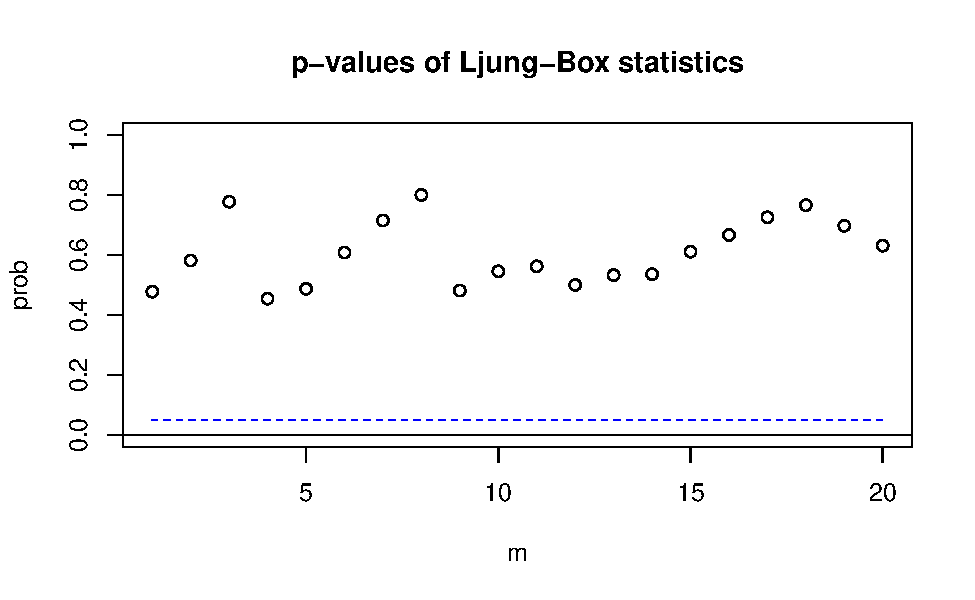
\includegraphics{exercise_1_files/figure-latex/unnamed-chunk-3-1.pdf}

\FloatBarrier

For this time series there are no autocorrelation for the first 20 lags.

Next, we will have a look at time series for \emph{Morgan Stanley (MS)}.
\FloatBarrier

\begin{Shaded}
\begin{Highlighting}[]
\KeywordTok{mq}\NormalTok{(}\DataTypeTok{x =}\NormalTok{ tenstocks}\OperatorTok{$}\NormalTok{MS, }\DataTypeTok{lag =} \DecValTok{20}\NormalTok{) }
\end{Highlighting}
\end{Shaded}

\begin{verbatim}
## Ljung-Box Statistics:  
##            m       Q(m)      df    p-value
##  [1,]  1.00000   0.00526  1.00000     0.94
##  [2,]  2.00000   1.24473  2.00000     0.54
##  [3,]  3.00000   1.42333  3.00000     0.70
##  [4,]  4.00000   1.42489  4.00000     0.84
##  [5,]  5.00000   2.91701  5.00000     0.71
##  [6,]  6.00000   3.47398  6.00000     0.75
##  [7,]  7.00000   4.30334  7.00000     0.74
##  [8,]  8.00000   6.89871  8.00000     0.55
##  [9,]  9.00000   7.55530  9.00000     0.58
## [10,] 10.00000   8.45013 10.00000     0.58
## [11,] 11.00000   8.89468 11.00000     0.63
## [12,] 12.00000   8.97639 12.00000     0.70
## [13,] 13.00000   9.72283 13.00000     0.72
## [14,] 14.00000   9.72714 14.00000     0.78
## [15,] 15.00000  10.75241 15.00000     0.77
## [16,] 16.00000  10.76237 16.00000     0.82
## [17,] 17.00000  15.18350 17.00000     0.58
## [18,] 18.00000  15.21323 18.00000     0.65
## [19,] 19.00000  17.13504 19.00000     0.58
## [20,] 20.00000  17.73024 20.00000     0.61
\end{verbatim}

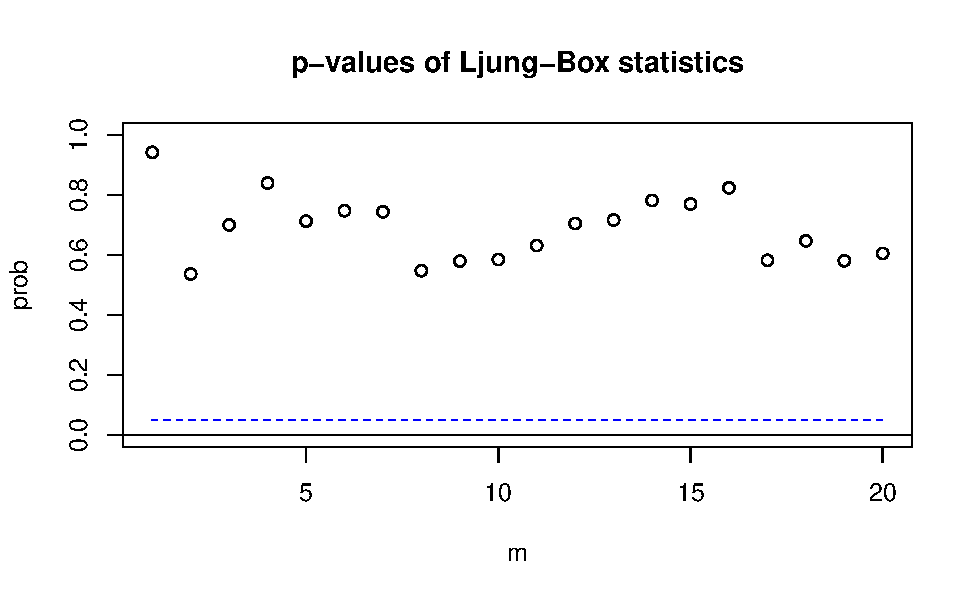
\includegraphics{exercise_1_files/figure-latex/unnamed-chunk-4-1.pdf}

The results for the \emph{MS} time series are similar to those of the
\emph{JPM}.

Lastly, there is only the time series from \emph{Goldman Sachs Group Inc
(GS)} left to be analysed.

\begin{Shaded}
\begin{Highlighting}[]
\KeywordTok{mq}\NormalTok{(}\DataTypeTok{x =}\NormalTok{ tenstocks}\OperatorTok{$}\NormalTok{GS, }\DataTypeTok{lag =} \DecValTok{20}\NormalTok{)}
\end{Highlighting}
\end{Shaded}

\begin{verbatim}
## Ljung-Box Statistics:  
##         m       Q(m)     df    p-value
##  [1,]  1.00      3.12    1.00     0.08
##  [2,]  2.00      3.12    2.00     0.21
##  [3,]  3.00      4.55    3.00     0.21
##  [4,]  4.00      4.94    4.00     0.29
##  [5,]  5.00      5.68    5.00     0.34
##  [6,]  6.00      7.13    6.00     0.31
##  [7,]  7.00      7.26    7.00     0.40
##  [8,]  8.00      7.34    8.00     0.50
##  [9,]  9.00      9.02    9.00     0.44
## [10,] 10.00      9.02   10.00     0.53
## [11,] 11.00      9.70   11.00     0.56
## [12,] 12.00     10.32   12.00     0.59
## [13,] 13.00     12.82   13.00     0.46
## [14,] 14.00     13.44   14.00     0.49
## [15,] 15.00     16.97   15.00     0.32
## [16,] 16.00     17.70   16.00     0.34
## [17,] 17.00     17.72   17.00     0.41
## [18,] 18.00     17.84   18.00     0.47
## [19,] 19.00     24.27   19.00     0.19
## [20,] 20.00     24.28   20.00     0.23
\end{verbatim}

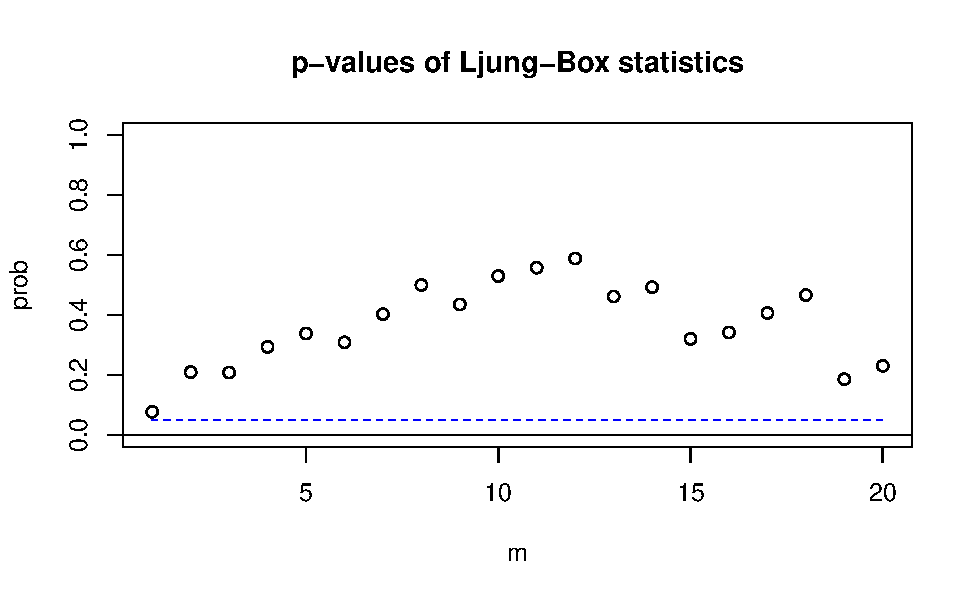
\includegraphics{exercise_1_files/figure-latex/unnamed-chunk-5-1.pdf}

Only the first lag is \emph{relatively} close to significant to a 5
percent significance level

\begin{itemize}
  \item[b)] $\quad$
\end {itemize}

Now we take a look at the combined test.

\begin{Shaded}
\begin{Highlighting}[]
\KeywordTok{mq}\NormalTok{(}\DataTypeTok{x =} \KeywordTok{cbind}\NormalTok{(tenstocks}\OperatorTok{$}\NormalTok{JPM, tenstocks}\OperatorTok{$}\NormalTok{MS, tenstocks}\OperatorTok{$}\NormalTok{GS), }\DataTypeTok{lag =} \DecValTok{20}\NormalTok{)}
\end{Highlighting}
\end{Shaded}

\begin{verbatim}
## Ljung-Box Statistics:  
##         m       Q(m)     df    p-value
##  [1,]   1.0      25.1     9.0     0.00
##  [2,]   2.0      33.6    18.0     0.01
##  [3,]   3.0      55.2    27.0     0.00
##  [4,]   4.0      78.1    36.0     0.00
##  [5,]   5.0      95.3    45.0     0.00
##  [6,]   6.0     103.4    54.0     0.00
##  [7,]   7.0     113.7    63.0     0.00
##  [8,]   8.0     122.9    72.0     0.00
##  [9,]   9.0     135.2    81.0     0.00
## [10,]  10.0     145.1    90.0     0.00
## [11,]  11.0     149.4    99.0     0.00
## [12,]  12.0     162.5   108.0     0.00
## [13,]  13.0     167.4   117.0     0.00
## [14,]  14.0     180.3   126.0     0.00
## [15,]  15.0     192.0   135.0     0.00
## [16,]  16.0     205.4   144.0     0.00
## [17,]  17.0     218.8   153.0     0.00
## [18,]  18.0     227.4   162.0     0.00
## [19,]  19.0     236.5   171.0     0.00
## [20,]  20.0     244.1   180.0     0.00
\end{verbatim}

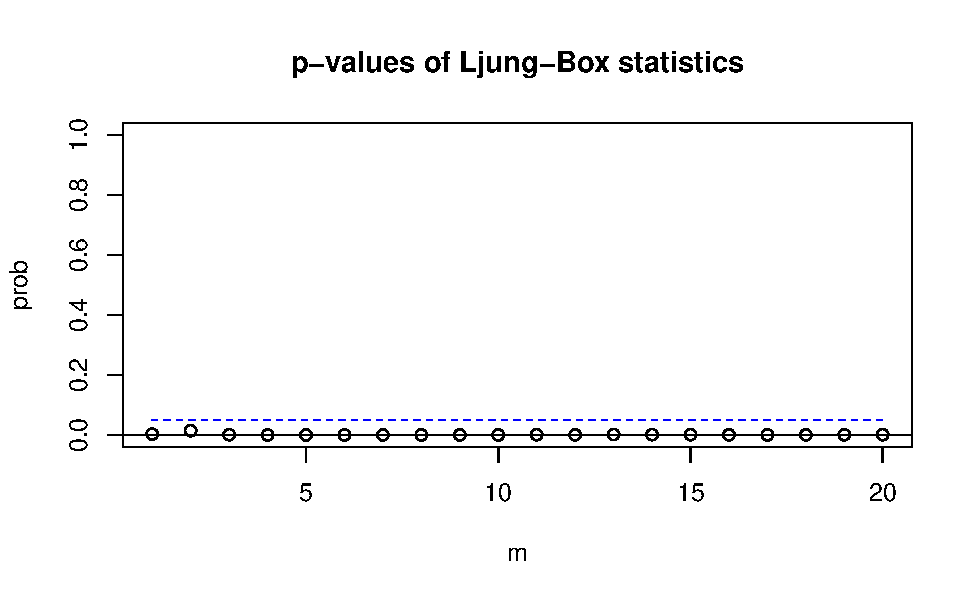
\includegraphics{exercise_1_files/figure-latex/unnamed-chunk-6-1.pdf}

All p-values are below 5\%. Since the time series are not much
autocorrelated (univariate!), there must be cross-correlations which
cause the Null hypothesis to be rejected. So there is a dynamic pattern
which might be explained using multivariate time series models.

Lets have a look at the correlation to may see some patterns.

\begin{Shaded}
\begin{Highlighting}[]
\KeywordTok{ccf}\NormalTok{(}\DataTypeTok{x =}\NormalTok{ tenstocks}\OperatorTok{$}\NormalTok{JPM, }\DataTypeTok{y =}\NormalTok{ tenstocks}\OperatorTok{$}\NormalTok{MS, }\DataTypeTok{lag.max =} \DecValTok{20}\NormalTok{)}
\KeywordTok{ccf}\NormalTok{(}\DataTypeTok{y =}\NormalTok{ tenstocks}\OperatorTok{$}\NormalTok{JPM, }\DataTypeTok{x =}\NormalTok{ tenstocks}\OperatorTok{$}\NormalTok{MS, }\DataTypeTok{lag.max =} \DecValTok{20}\NormalTok{) }
\KeywordTok{ccf}\NormalTok{(}\DataTypeTok{x =}\NormalTok{ tenstocks}\OperatorTok{$}\NormalTok{JPM, }\DataTypeTok{y =}\NormalTok{ tenstocks}\OperatorTok{$}\NormalTok{GS, }\DataTypeTok{lag.max =} \DecValTok{20}\NormalTok{)}
\KeywordTok{ccf}\NormalTok{(}\DataTypeTok{x =}\NormalTok{ tenstocks}\OperatorTok{$}\NormalTok{MS, }\DataTypeTok{y =}\NormalTok{ tenstocks}\OperatorTok{$}\NormalTok{GS, }\DataTypeTok{lag.max =} \DecValTok{20}\NormalTok{)}
\end{Highlighting}
\end{Shaded}

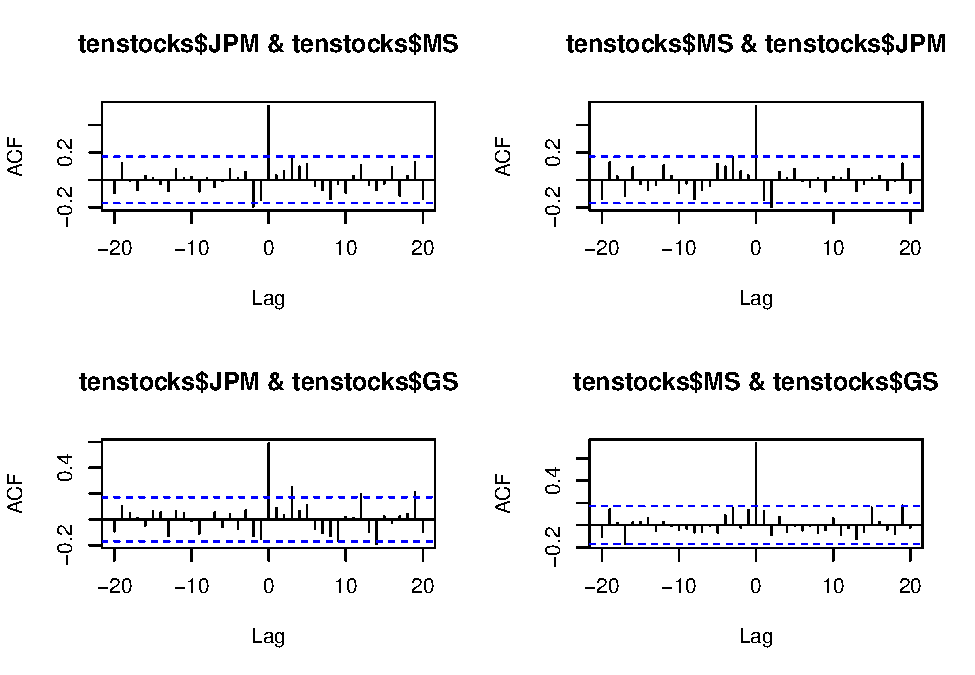
\includegraphics{exercise_1_files/figure-latex/unnamed-chunk-8-1.pdf}

But keep in mind that the \emph{Ljung-Box} test does not take \(\rho_0\)
into consideration. Lastly, we will plot the times series with the
command \texttt{plot.ts()}.

\begin{Shaded}
\begin{Highlighting}[]
\KeywordTok{plot.ts}\NormalTok{(}\KeywordTok{cbind}\NormalTok{(tenstocks}\OperatorTok{$}\NormalTok{JPM, tenstocks}\OperatorTok{$}\NormalTok{MS, tenstocks}\OperatorTok{$}\NormalTok{GS)) }
\end{Highlighting}
\end{Shaded}

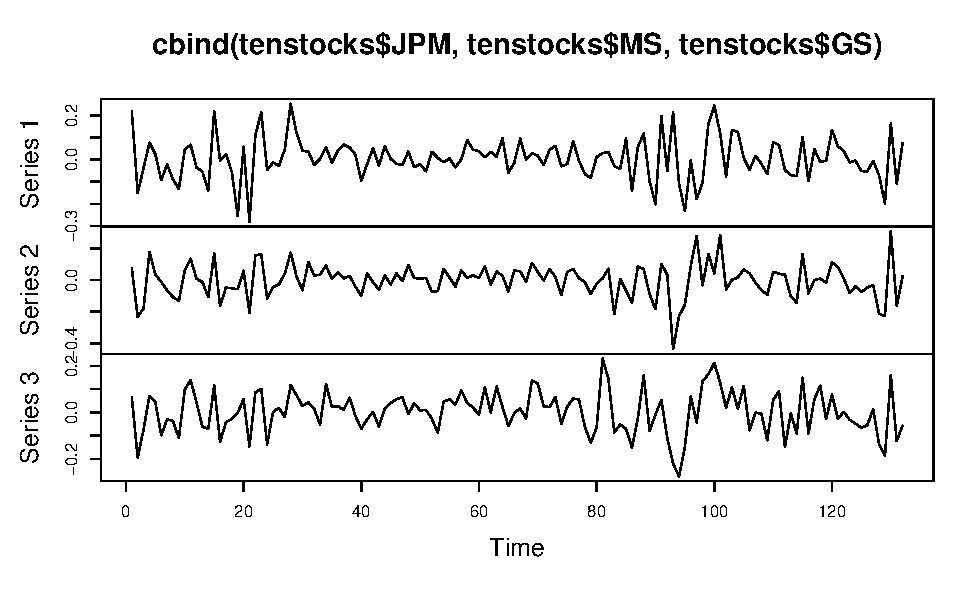
\includegraphics{exercise_1_files/figure-latex/unnamed-chunk-9-1.pdf}

\end{document}
